% Time-stamp: <09/10/02 01:57:13 vilhuber>
% $Id: Presentation-PSD.tex 3219 2012-09-27 07:47:11Z vilhu001 $

% normal line:
\documentclass[xcolor=table,compress]{beamer}
% to create notes:
%\documentclass[handout,notes=only]{beamer}
% to create handouts
%\documentclass[xcolor=table,handout,compress]{beamer}
% to create a different kind of handouts
%\documentclass{article}
%\usepackage[envcountsect]{beamerarticle}

%\setbeameroption{handout}
%\setbeameroption{show notes}


%
% Packages
%
\mode<article> % only for the article version
{
  \usepackage{fullpage}
  \usepackage{hyperref}
}
\usepackage{ifpdf}
\ifpdf
\usepackage{embedfile}
\embedfile{\jobname.tex}
\fi

\usepackage{graphicx}
%\usepackage{pstricks}
\usepackage{xcolor}
\usepackage{pifont}
%\usepackage{../chicago}
\usepackage{pgf}
\usepackage{amsmath,amssymb,amsfonts}
\usepackage[latin1]{inputenc}
\usepackage{colortbl}
\usepackage[english]{babel}
\usepackage{array}
\usepackage{pdfpages}
% usage:
%   \includepdf[pages={1}]{myfile.pdf}
%   \includepdf[pages={1,3,5}]{myfile.pdf} would include pages 1, 3, and 5 of the file. 
%   To include the entire file, you specify pages={-}, where {-}
%\usepackage{landscape}
\usepackage{listings}
\lstloadlanguages{R,bash}
\lstset{numbers=left, stepnumber=1,  language=bash, basicstyle=\tiny}

%\usepackage{lmodern}
%\usepackage[T1]{fontenc}

\usepackage{times}
%\usepackage{colortbl}

%============================================================
% Beamer specific styles and configs
%============================================================

\mode<presentation>
{
% alternative, could always use
%\usetheme{Census}
\usetheme{cornell}
\useoutertheme{cornell}
}


%\setbeamercovered{dynamic}



%============================================================
% Title
%============================================================

\title[Computing for Economists]{Workshop: High-performance computing for economists}
\author[Vilhuber, Abowd, Mansfield, McKinney]{%
  Lars~Vilhuber\inst{1} \and
  John M. Abowd\inst{1} \and
  Richard~Mansfield\inst{1} \and
  Kevin~L.~McKinney %\inst{2}%
}

\institute[Cornell]{
  \inst{1}%
   Cornell University, Economics Department,
%\and \inst{2} U.S. Census Bureau
}%
\date[Aug 17-19, 2015]{August 17-19, 2015}
\subject{HPC}


% % % % % % % % % % % % % % % % % Main document
\begin{document}
\frame{\titlepage}
\section{Getting access to ECCO}


\begin{frame}{Getting access to ECCO}
\begin{block}{You already have...}
\begin{itemize}
\item You have an account by virtue of participating in this class
\item Moving forward, you will be eligible to faculty-sponsored accounts
\item Currently soft-monitoring of resource usage
\end{itemize}
\end{block}
\pause
\begin{block}{... but do you have \textbf{access}?}
Have you logged in via SSH to reset your password? \newline \uncover<3->{\alert{$\rightarrow$ 
\href{http://www2.vrdc.cornell.edu/news/ecco/step-2-first-login/}{Instructions}}}
\end{block}
\end{frame}


\begin{frame}{Quick walkthrough, using Chrome SSH}
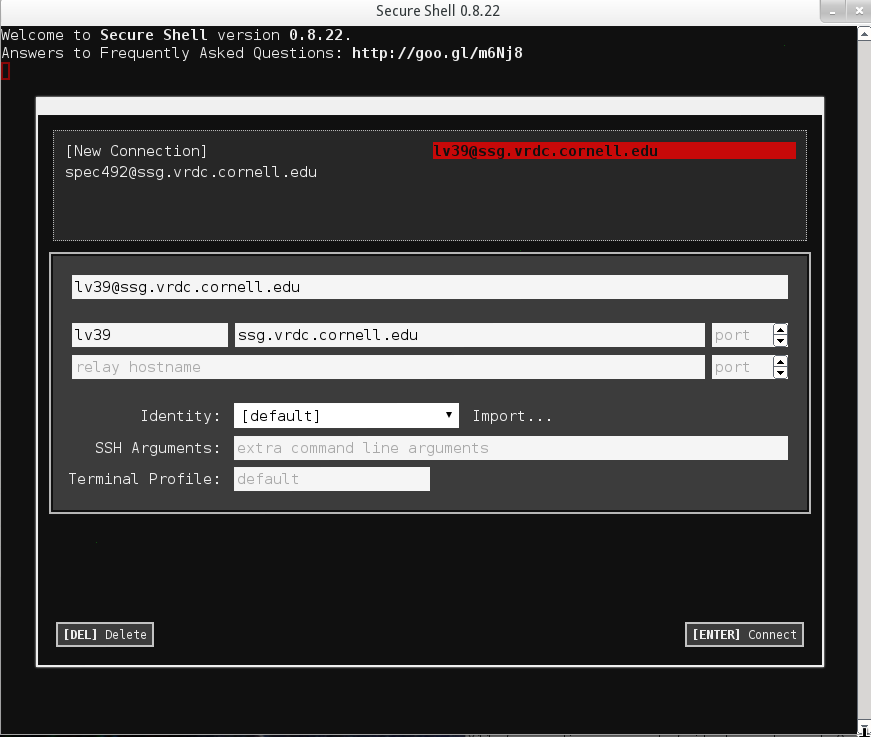
\includegraphics[width=.9\textwidth]{chrome-ssh-screen1.png}
\end{frame}


\begin{frame}{Quick walkthrough, using Chrome SSH}
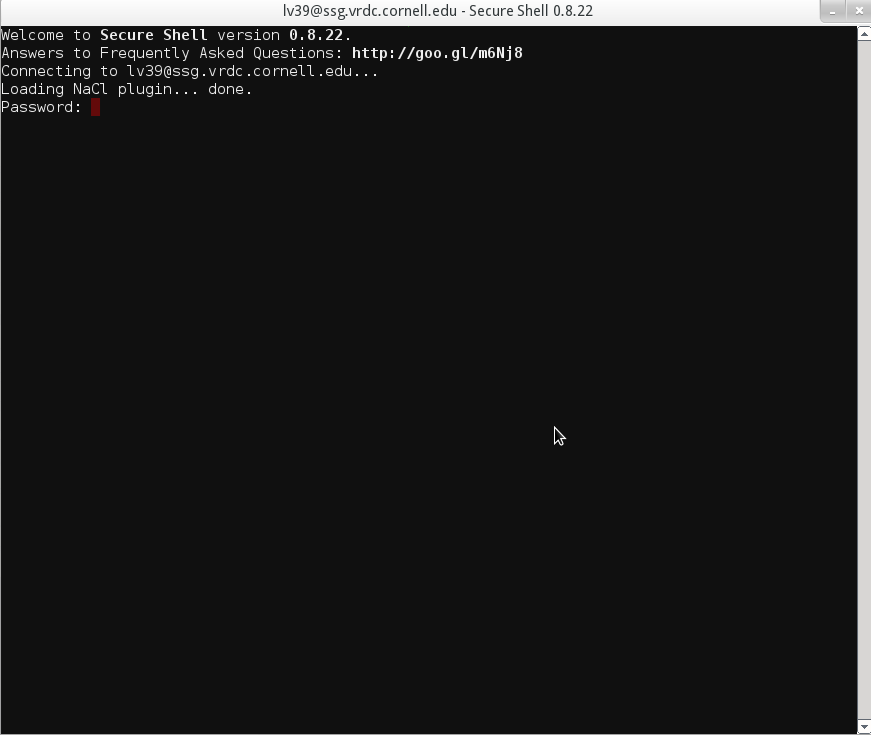
\includegraphics[width=.9\textwidth]{chrome-ssh-screen2.png}
\end{frame}


\begin{frame}{Quick walkthrough, using Chrome SSH}
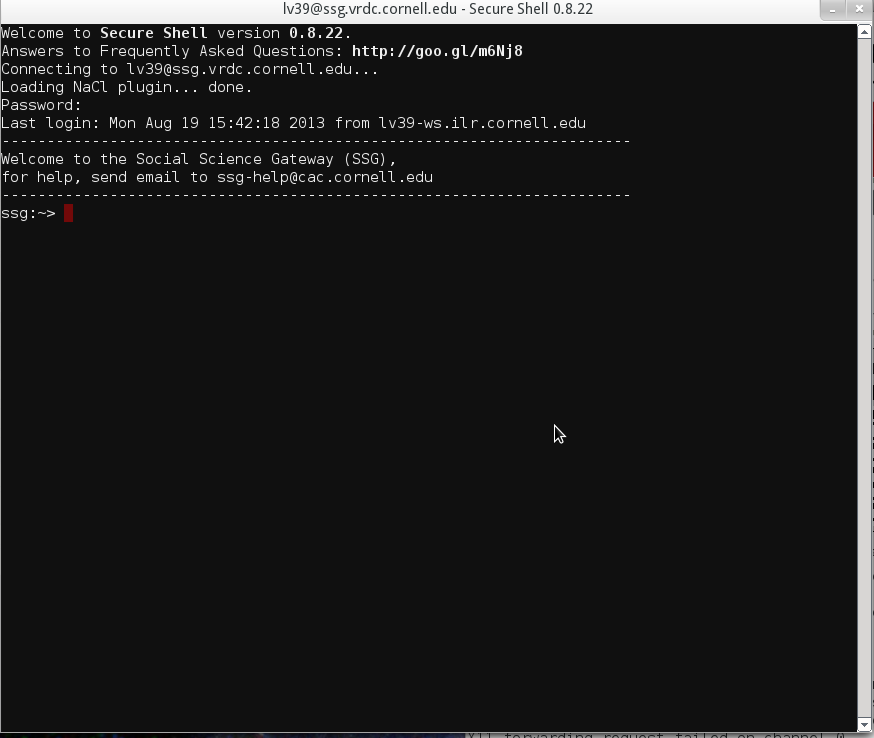
\includegraphics[width=.9\textwidth]{chrome-ssh-screen3.png}
\end{frame}



\begin{frame}{Access via NX}
\begin{block}{What is NX?}
NX is software similar to Windows Remote Desktop, allowing for a graphical interface to be made 
available remotely.
\end{block}
\begin{itemize}
\item Client is free (provided by Nomachine)
%\item We use a free server (not provided by Nomachine, but fully functional)
\item Clients can be launched by installing dedicated client (all OS)  
%or by launching the  webclient (currently not working for some Linux)
\end{itemize}
\end{frame}


\begin{frame}{Important note}
\begin{block}{NX on ECCO security}
You MUST download the custom-configured session from the VRDC website; the default session 
configuration from the NX client install will not work.
\end{block}
\tiny Details: we use a custom SSH key for the NX client, for some minimal additional security.
\end{frame}

\begin{frame}{Important note}
\begin{block}{Live demonstration}
This section is usually demoed live. The slides here may not correspond to the latest NX 
implementation on ECCO.
\end{block}

\end{frame}

\begin{frame}{Important note}
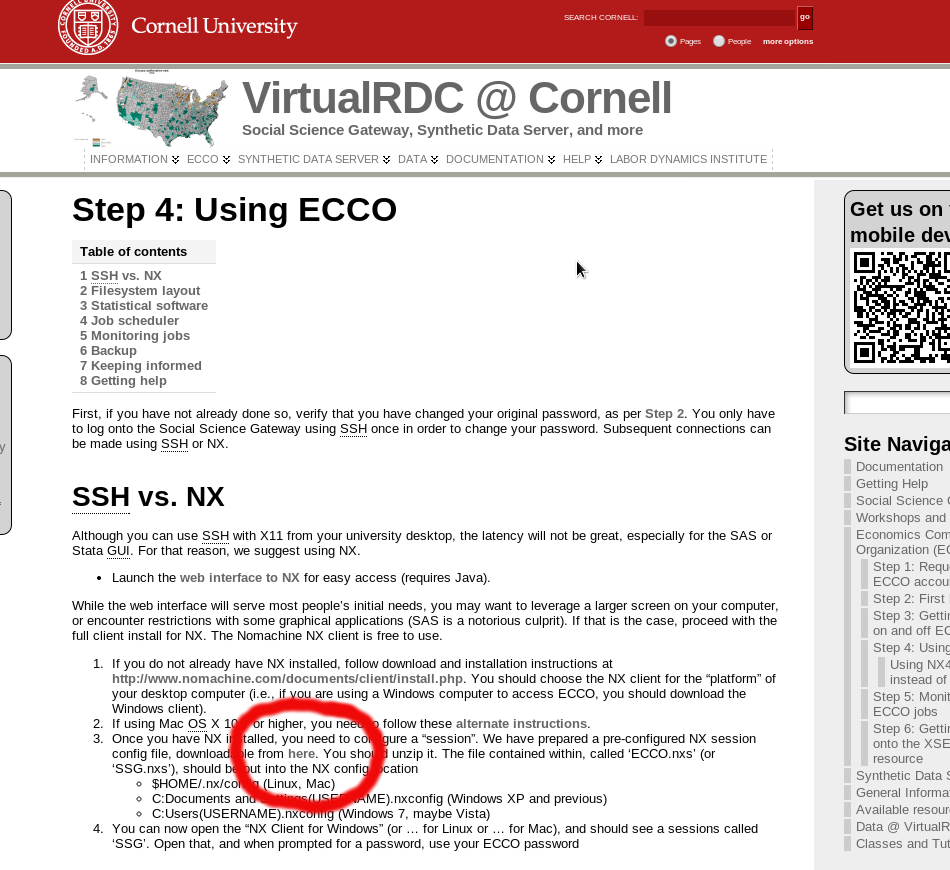
\includegraphics[height=.7\textheight]{nx-ecco-key.png}
\end{frame}


\begin{frame}{Logging on}
\centering
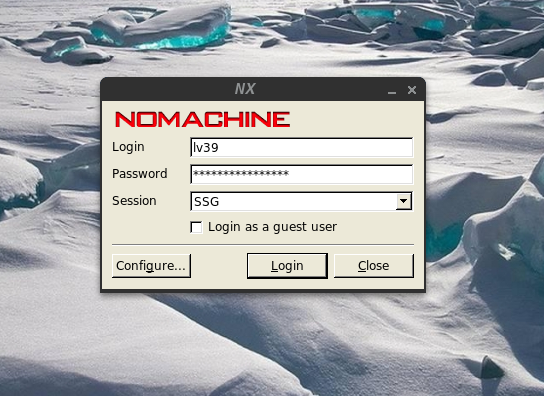
\includegraphics[height=.7\textheight]{nx-login-box.png}
\end{frame}


\begin{frame}{Successful connection}
\centering
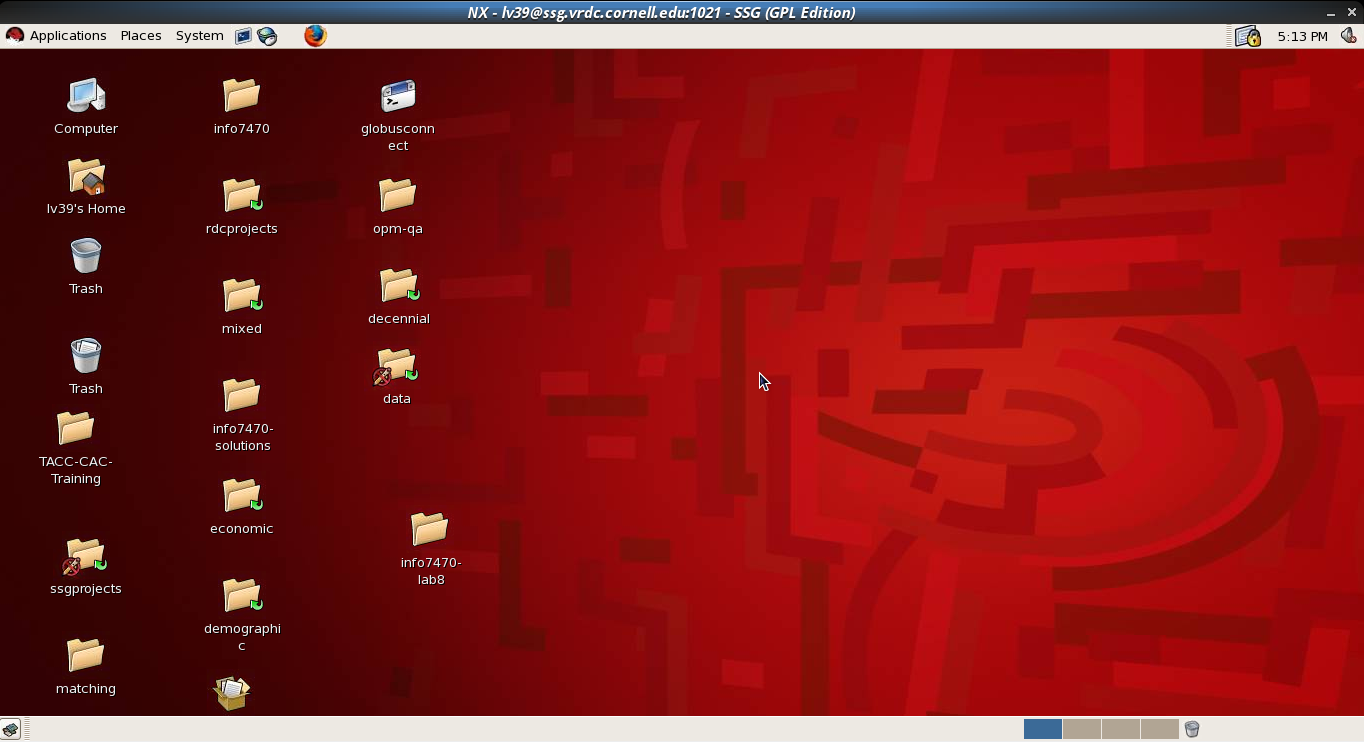
\includegraphics[width=1\textheight]{nx-logged-on.png}
\end{frame}


%\section[Data mgmt]{Considerations for data management}
%\begin{frame}
%\href{day3-2.pdf}{Data management}
%\end{frame}
%\section[Basics]{Basics of High-performance computing}
%\begin{frame}
%\href{day3-3.pdf}{Basics}
%\end{frame}
%
%
%\section{Wrap up}
%
%\begin{frame}
%\href{day3-4.pdf}{Wrap-up}
%\end{frame}

\end{document}